\section{Implementation \& Design}
  For this paper the Fibonacci and the Sort algorithm from BOTS are chosen to be implemented, as introduced in subsection \ref{subsec:BOTS}.
  Additionally, a generic algorithm is implemented.
  All three are implemented using OpenMP, HPX and in a sequential way.
  
  \paragraph{Fibonacci}
  The algorithm can spawn a high amount of tasks with small workload.
  The workload of forking and joining new threads might have the biggest impact when it comes to performance.
  
  The implementation is done without cut offs for the HPX and OpenMP versions.
  This means that every recursive call of the Fibonacci function creates a new task.
  \begin{lstlisting}[
  caption=Fibonacci OpenMP Implementation,
  label=lst1:fibOMP,
]
long long fibonacci(long long input) {
    if (input < 2 ) return input;
    long long x, y;
    #pragma omp task shared(x) firstprivate(input)
    x = fibonacci(input - 1);
    #pragma omp task shared(y) firstprivate(input)
    y = fibonacci(input - 2);
    #pragma omp taskwait
    return x + y;
}
\end{lstlisting}
  Listing \ref{lst1:fibOMP} shows a first implementation of the Fibonacci algorithm using OpenMP.
  It shows which directives are used.
  As explained in subsection \ref{subsec:OpenMP}, the \texttt{\#pragma omp task} directive creates a new task which may be executed.
  Using the \texttt{shared} and \texttt{firstprivate} clauses adjusts the variable scopes so that each task has its own instance of the parameter input.
  Variables \texttt{x} and \texttt{y} are shared which means no new instance is created.
  At the end the \texttt{\#pragma omp taskwait} directive tells the function to wait until all the child tasks finished their execution.
  
\begin{lstlisting}[
  caption=Fibonacci HPX Implementation,
  label=lst1:fibHPX,
]
long long fibonacci(long long input) {
  if (input < 2) return input;
  hpx::future<long long> n1 =
      hpx::async(fibonacci, input - 1);
  long long n2 = fibonacci(input - 2);
  return n1.get() + n2;
}
\end{lstlisting}
  The HPX implementation of the Fibonacci algorithm can be seen in listing \ref{lst1:fibHPX}.
  In contrast to OpenMP, HPX works with futures to abstract results of function calls.
  Calling a function with \texttt{hpx::async} creates a task and immediately returns a future to continue the execution.
  Calling \texttt{get} on a future suspends the current thread until this future is returned.
\begin{figure}[htbp]
	\centering
	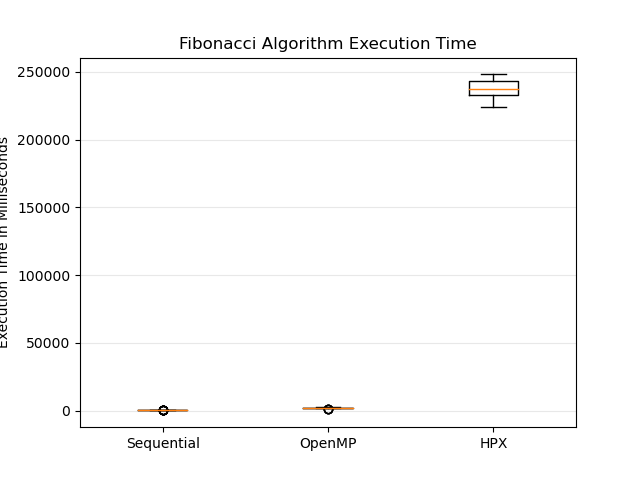
\includegraphics[width=0.45\textwidth]{figures/fib_NoOp.png}
	\caption{Execution times of the Fibonacci algorithm}
	\label{fig:fib_NoOp}
\end{figure}

- 22 fibonacci number
  \\
 
  \paragraph{Merge Sort}
  The Sort algorithm of BOTS is slightly adjusted to a normal merge sort.
  It is a suitable use case, easy to implement and can also spawn a high number of tasks.
  Also in case of merge sort no cut off is implemented.
  \begin{figure}[htbp]
	\centering
	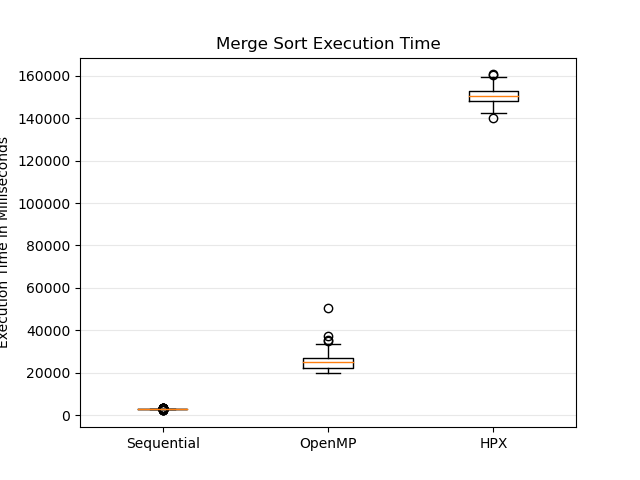
\includegraphics[width=0.45\textwidth]{figures/sort_NoOp.png}
	\caption{Execution times of Merge Sort}
	\label{fig:sort_NoOp}
  \end{figure}
  The measurements of figure \ref{fig:sort_NoOp} are created on environment three and show the average of 100 runs.
  The merge sort is run on 10.000 random elements which are created in a deterministic way.
  Similar to Fibonacci, merge sort also creates a lot of tasks and HPX shows the slowest execution time.
  Sequential has the shortest average time and the OpenMP average times differ more significantly this time compared to the Fibonacci example. 
  \\
  
  \paragraph{Generic Algorithm}
  The aim of this algorithm is to enable task size adjustment and allow to define the number of tasks.
  
  The algorithm uses two vectors which sizes are defined at the building process.
  Suggested is a size of 1024 for each.
  First of all one vector is filled by randomized floating point numbers.
  To compare each run a deterministic seed for the random numbers is chosen.
  In each turn the element of a vector is equal to a calculation on the element of the other vector.
  The sinus function is calculated on the element before it is multiplied by ten and adjusted to an absolute value.
  This turns are repeated a defined number of times.
  After the last turn is executed, each elements of the last calculated vector are summed up.
  
  The task size can be adapted by parameters and defines how many vector elements are calculated by a task.
  The task size furthermore defines how many tasks are used per run.
  This number is equal to the vector size divided by the task size.
  As each turn depends on the execution of the previous turn, the number of dependencies can be increased by using more tasks per turn.
\begin{figure}[htbp]
	\centering
	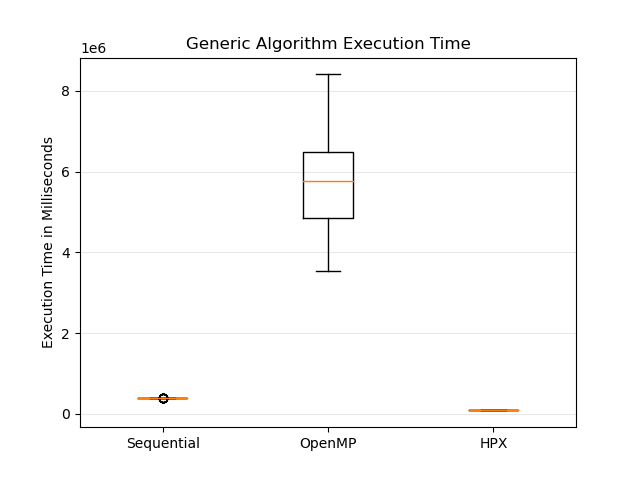
\includegraphics[width=0.45\textwidth]{figures/generic_NoOp.png}
	\caption{Execution times of the generic algorithm}
	\label{fig:gen_NoOp}
\end{figure}

Figure \ref{fig:gen_NoOp} shows the measured execution times for the generic algorithm in his three versions.
Again these are the average values of 100 runs on the system of environment three.
20 turns are made with a task size of 20 and the array size is 1,048,576.
It can be seen that the range of OpenMP times is quite big compared to the sequential and HPX version.
Additionally, the OpenMP version takes the longest time to complete the execution whereas HPX is the fastest of these three. 
		
\subsection{Optimization}
  On possible optimization used in the BOTS benchmarks and mentioned in \cite{LaGrone.2011} is to use the cutoff option.
  This can be achieved by using if clause which is provided by the task directive.
  In case this clause evaluates to false no task will be spawned and the execution continues with the function call.
  \textbf{TODO: CUT OFF RESULTS -- USE BOTS CODE}
   
  Another optimization approach might be to see if there is a difference in using tied or untied tasks.
  Untied tasks improve the load balancing as each free thread can start executing a task which is ready to be executed.
  The disadvantage of untied tasks is that the data is not always available locally.
  This means in case a thread wants to execute a ready task which is not created by it, the data and context has to be transferred to new execution location.
  \textbf{TODO: UNTIED VS TIED TASKS}	
	
		
    
    
    \cite{MKlemm.2018}
 --> directives to optimize
 	-->taskyield - suspend the current task in favor of execution of a different task
 	--> if - in case it is false the task is executed immediately
 	--> mergeable - A task for which the data environment, is the same as that of its generating task region
 	--> final - force all child tasks to become final and included
 		--> if true --> child tasks become included --> means that the tasks are also executed by the parent task

  \cite{TheSTEARGroup.2020}
    - HPX --> Performance counters to identify bottlenecks
    - HPX exposes special API functions to allow one to create, manage and read the counter data
    - all performance counter instances have a unique name to access the counter


  \cite{hpxMP.2019}
  \cite{TheSTEARGroup.2020}
    - HPX supports 7 different thread scheduling policies:
      - priority scheduling /default: 1 high priority and 1 low priority queue Queue per OS thread
      - static priority scheduling: 1 low and 1 high prio queue per OS thread --> round robin used in queue
      - local scheduling: 1 queue per per OS thread
      - static scheduling: 1 queue per OS thread --> round robin
      - global scheduling: one shared queue
      - ABP scheduling: double ended lock-free queue per OS thread --> insert threads on top and steal threads from bottom
      - Hierarchy scheduling: tree of task items, each OS Thread traverses through to obtain new task item
      - Periodic priority scheduling: 1 queue of task items per OS thread, couple of high priority queues and one low priority queue
      